\section{L-systémy}\label{sec:L-systemy}

Uvedeme tuto kapitolu s~ohledem na předchozí obsah trochu netradičně a od matematiky se (alespoň zdánlivě) na chvíli odkloníme. Podíváme se na fraktály,~s jejichž způsobem popisu přišel roku 1968 maďarský biolog \name{Aristid Lindenmayer} (1925--1989) a který (možná pro někoho i~překvapivě) má základy především v~informatice. \citep[str. 2]{Prusinkiewicz1990}

K popisu specifického druhu fraktálů lze využít znalosti z \emph{teorie formálních jazyků} a \emph{teorie automatů}, na jejímž počátku stál (mj.) britský matematik a informatik \name{Alan Turing} (1912--1954). Ten ve svém článku \emph{On Computable Numbers, with an Application to the Entscheidungsproblem} z roku 1936 zavedl koncept abstraktního stroje dnes známého jako \emph{Turingův stroj}\index{Turingův stroj}, jednoduché zařízení s výpočetními schopnostmi již tehdy porovnatelnými se současnými počítači.
\begin{figure}[h]
    \centering
    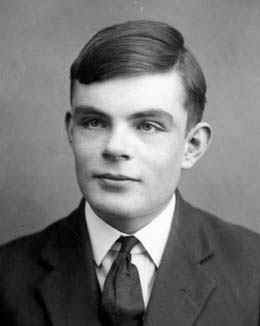
\includegraphics[width=.4\textwidth]{Alan-Turing.jpeg}
    \caption[Alan Turing,~1871--1956]{Alan Turing\footnote{Převzato z~\cite{OConnorTuring2025}},~1912--1954}
    \label{fig:alan-turing}
\end{figure}
V té době se zabýval otázkou, kterou v roce 1928 položil známý německý matematik \name{David Hilbert} (1862--1943), jež je známá pod názvem \emph{"Entscheidungsproblem"}\index{Entscheidungsproblem}\footnote{Anglicky \emph{The Decision problem}\index{The Decision problem}, česky přeložitelné jako \emph{"rozhodovací problém"}. Zde však poznamenejme, že onem český termín se používá i v související teorii složitosti a vyčíslitelnosti, má však podstatně jiný význam.}. Problémem bylo, zda existuje algoritmus, který o každém tvrzení je schopný rozhodnout (v konečném čase), zda je či není pravdivé. Později Alan Turing tento problém přeformuloval takto: \emph{Existuje program, který o jiném programu na vstupu rozhodne, zda se zastaví, či nikoliv?} David Hilbert byl ve svých vizích optimistický, avšak nakonec Alan Turing dokázal, že \textbf{takový algoritmus nemůže existovat}. Způsob, jakým Turing došel onomu výsledku, byl v konečném důsledku vlastně až překvapivě jednoduchý a existuje pro něj velké množství popularizačních materiálů\footnote{Pokud by se chtěl čtenář dozvědět více o této problematice a teorii s ní související, doporučuji např. knihu \cite{Motwani2003}}.
\begin{figure}[h]
    \centering
    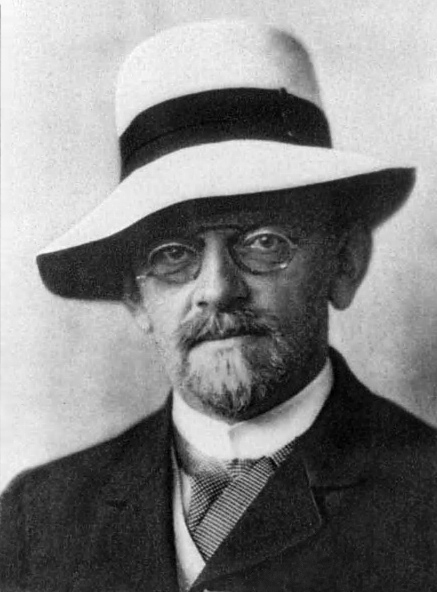
\includegraphics[width=.4\textwidth]{David-Hilbert.jpg}
    \caption[David Hilbert,~1871--1956]{David Hilbert\footnote{Převzato z~\cite{OConnorHilbert2025}},~1862--1943}
    \label{fig:david-hilbert}
\end{figure}